\section{Requirements}

\subsection{User Stories}
\begin{comment}
Use the template from the course website and list all user stories here. It is
fine to have them in an spreadsheet (or other applications, such as Trello) at
first, but they must end up here as well.

These user stories should describe what the user will be able to do. Write
the user stories in language of the customer, and give them a unique ID. List
the user stories in order of priority.

You need to annotate an user story whether or not it is implemented. We need to
know which user stories are implemented, such that we can check this during the
oral presentation.
\end{comment}


\UserStory{1}{Move around the world\\\D}{As an explorer i want to be able to to move around in the world so i can see new places}
{\begin{itemize}[+]
	\item Change location of player character.
	\item Move player according to input.
	\item Animation when walking.
	\item Animation when standing still.
\end{itemize}}
\UserStory{2}{See the enviorment\\\D}{As a player i want to see my environment so I know where I am}
{\begin{itemize}[+]
	\item Parse tile sets.
	\item Implement map renderer class
\end{itemize}}
\UserStory{3}{Read inputs\\\D}{As a user I want the game to understand my inputs so I can play the game}
{\begin{itemize}[+]
	\item Implement an input listener
	\item Make input listener take input from keyboard
	\item Connect Input to model
\end{itemize}}
\UserStory{4}{Parse mapse\\\D}{As a modder, I want to be able to parse and make my own Tiled maps}
{\begin{itemize}[+]
	\item Load tile sets from Tiled file
	\item Load tile information from Tiled file
\end{itemize}}
\UserStory{5}{Handle collitions\\\D}{As a user, I want the world to limit my movements so I cant't walk through walls}
{\begin{itemize}[+]
	\item Implement collision logic
	\item Parse collision from a map file
\end{itemize}}
\UserStory{6}{Combat Monsters \\\D}{As a user, I want to be able to fight enemys}
{\begin{itemize}[+]
	\item Design combat interface
	\item Create a combat scene
\end{itemize}
}
\UserStory{7}{Encounter Monsters \\\D}{As a user, I want to be able to fine a monster to attack}
{\begin{itemize}[+]
	\item Encounters to trigger a new combat
	\item Change scene to view combat
\end{itemize}}
\UserStory{8}{Attack Monsters\\\D}{As a player i want my monsters to be able to attack, so I can win against other monsters.}{\begin{itemize}[+]
	\item Create an attack handler witch handles attacks
	\item Create a way for monsters to take damage
	\item Design health interface
	\item Implement health interface
\end{itemize}}
\UserStory{9}{Transition between maps\\\D}{As an explorer i want to be able to transition between different maps, so that i'm not stuck in the same area}{\begin{itemize}[+]
	\item Update Map not to be static and use a map manager instead
	\item Do the same thing as above for texture map
	\item Create multiple maps
	\item Update parser to use map transition data
	\item Transition logically
	\item Make TextureMapManager observe model MapManager for changing map
\end{itemize}}
\UserStory{10}{Escape combat\\\D}{As a pacifist I want to be able to run from combat so my monsters don't get hurt}{\begin{itemize}[+]
	\item Run action in combat menu
	\item Chance to end combat when running away
\end{itemize}}
\UserStory{11}{Differnt attacks in combat}{As a player, I want to be able to pick an attack so that I can strategically control my monster during combat}
{\begin{itemize}[+]
	\item Design a "pick an attack"- interface
	\item Implement visuals fo said interface
	\item Create several (more then one) different attacks to choice from
\end{itemize}}
\UserStory{12}{Collect multiple monsters}{As a user, I want to keep multiple monster with me so that I can use more then one}
{\begin{itemize}[+]
	\item Implement somewhere to store multiple monsters
	\item Design an interface for seeing your monsters
	\item Pick one that is the current one
\end{itemize}}
\UserStory{13}{Befriend monsters}{As a user, I want to befriend my enemies so I can have more friends}
{\begin{itemize}[+]
	\item Design a befriend interface
	\item Add befriending difficulty to monsters
	\item Display befriending difficulty in combat
	\item Add befriended monster to you monster party
\end{itemize}}
\UserStory{14}{Run faster}{As a user, I want to be able to run around in the world so I can move where i want faster.}
{\begin{itemize}[+]
	\item Optional faster movement
	\item New input to trigger faster movement
	\item New animation for faster movement
\end{itemize}}
\UserStory{15}{Ambient sound}{As a user, I want ambient sound so i can be immersed in the game.}
{\begin{itemize}[+]
	\item Implement sound player
	\item Change sound depending on environment
	\item Sound toggle/ volume control
\end{itemize}}
\UserStory{16}{Combat sound effects}{As a player, I want sound feedback from engaging monsters in combat}
{\begin{itemize}[+]
	\item Play sound according to action taken
	\item Play combat music to set the mood
	\item Play sound depending on hit or miss of attack
\end{itemize}}
\UserStory{17}{Populate the world}{As a user, I want NPC:s that i can talk to so that i feel less alone}
{\begin{itemize}[+]
	\item Non playable characters (NPC) rendered on screen
	\item interaction input
	\item Text for NPC to say
	\item Text shows up on screen
	\item The player can continue the text (so more is shown or it disappears)
\end{itemize}}
\UserStory{18}{Items}{As a user, I want consumables to help me fight monsters so that i can prepare more for combat}
{\begin{itemize}[+]
	\item Design consumable interface
	\item Create regenerative consumables
	\item Create damaging consumables.
\end{itemize}}



\subsection{Definition of Done}
\begin{comment}
In this section you list the acceptance criteria that are common for all user
stories. For example, the code should reviewed and tests, it should be under
version control, etc.
\end{comment}
The project code was structured in such a way that when a person felt that they were done with a user story,
they had to get it reviewed and be questioned about it by at least one other contributor.
The purpose of this practice was not only to make sure that the user story was implemented fully,
that can be done with tests, but to iron out code smells and to keep the code somewhat coherent and similar-looking throughout the project.

\subsection{User interface}
\begin{comment}
Include sketches, drawings and explanations of the application's user interface.
Describe the navigation between the different views.
\end{comment}
Feyrune's UI is split into two major parts, the combat view and the overworld view, where the combat view is used to represent and control encounters between the player and all of Feyrune's different creatures, and the overworld view manages how the player moves on the game map and the exploration aspect of the game.\\
\\
\subsubsection{Combat view}
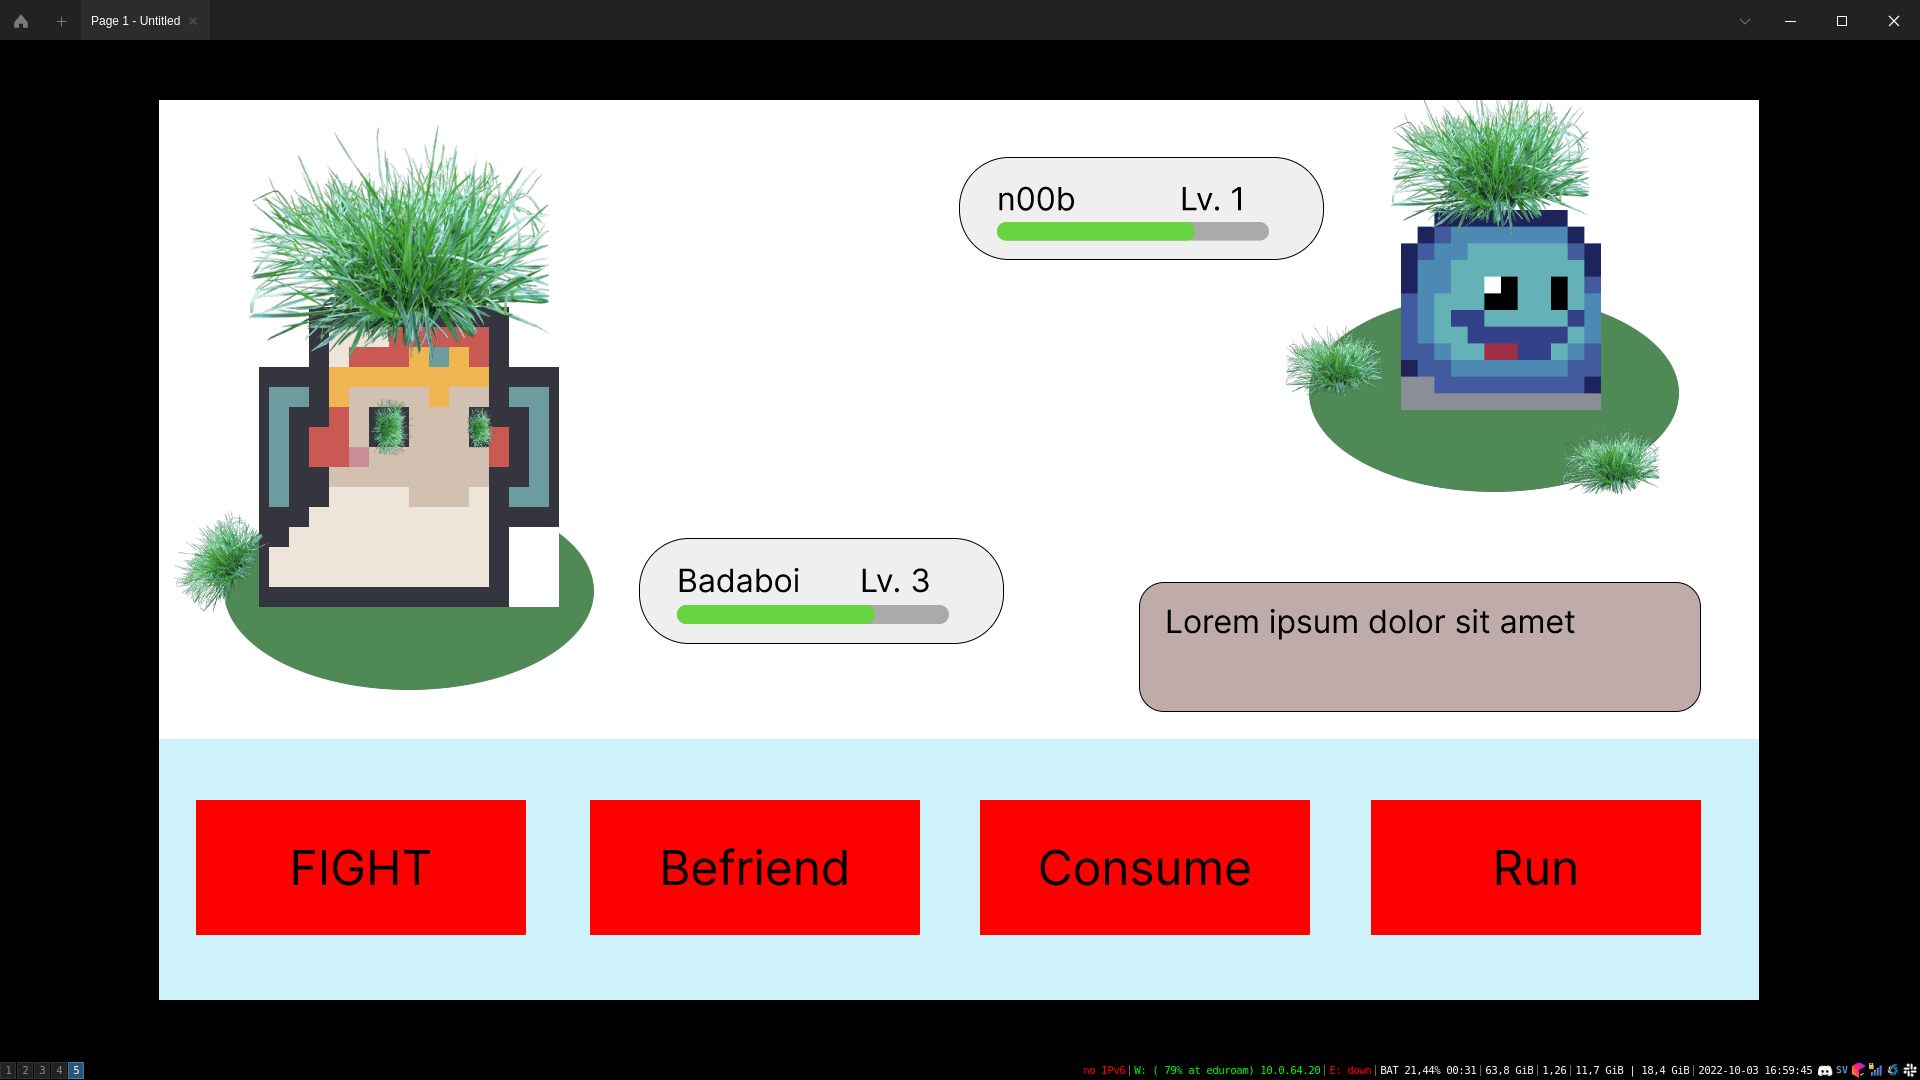
\includegraphics[width=\textwidth]{images/combat_figma.png}\\
The combat view in Feyrune is inspired by the Pokémon video games, sharing many familiar characteristics. It has four buttons at the bottom of the screen, one for changing the currently used player monster, one for attacking, another for fleeing and a last one for deciding to use an item.\\
\\
When clicking any of these buttons the menu will change to show the options available for that action. The player monster button will show the player's monsters, and the player can choose which one to use. The attack button will show the attacks available for the currently selected player monster. The item button will show the items available for use. The flee button however, immediately executes the action to flee, as it cannot be done in multiple different ways. At which point the player would be sent back to the overworld.\\
\\
The combat view shows the player and enemy creatures in the middle of the screen using sprites, and their health using green bars at the top of the screen to help the player see the current status of the battle. If the player creature "dies" during combat, the player gets sent back to the bed in the beginning of the bed.\\
\\
\subsubsection{Overworld view}
The overworld view in Feyrune is highly inspired from Nintendo games such as "The Legend of Zelda" and "Pokémon Pearl". The view consists of two different layers; a background layer displaying the ground of the map, whether it's made of grass or stone or something completely different, and a foreground layer displaying the player character and any other items visible, such as trees or benches.\\
%Insert image of one of the maps here
\\
The player character is represented by a sprite, and the player can move the character around the map by using the WASD control scheme. Feyrune includes no form of tooltips or other hints to which buttons to press to do what, as the game is meant to be played on a keyboard, and most player should be familiar with the WASD control scheme.\\
\\
When a player in the overworld enter a tile containing an encounter, something without a graphical representation as to create a feeling of randomness and suspense, the player will be moved to the combat view, where they can fight the creature they have just encountered.\\